% !TEX root = ../main.tex
\begin{figure}[t]
  \centering
  \iflatexml
  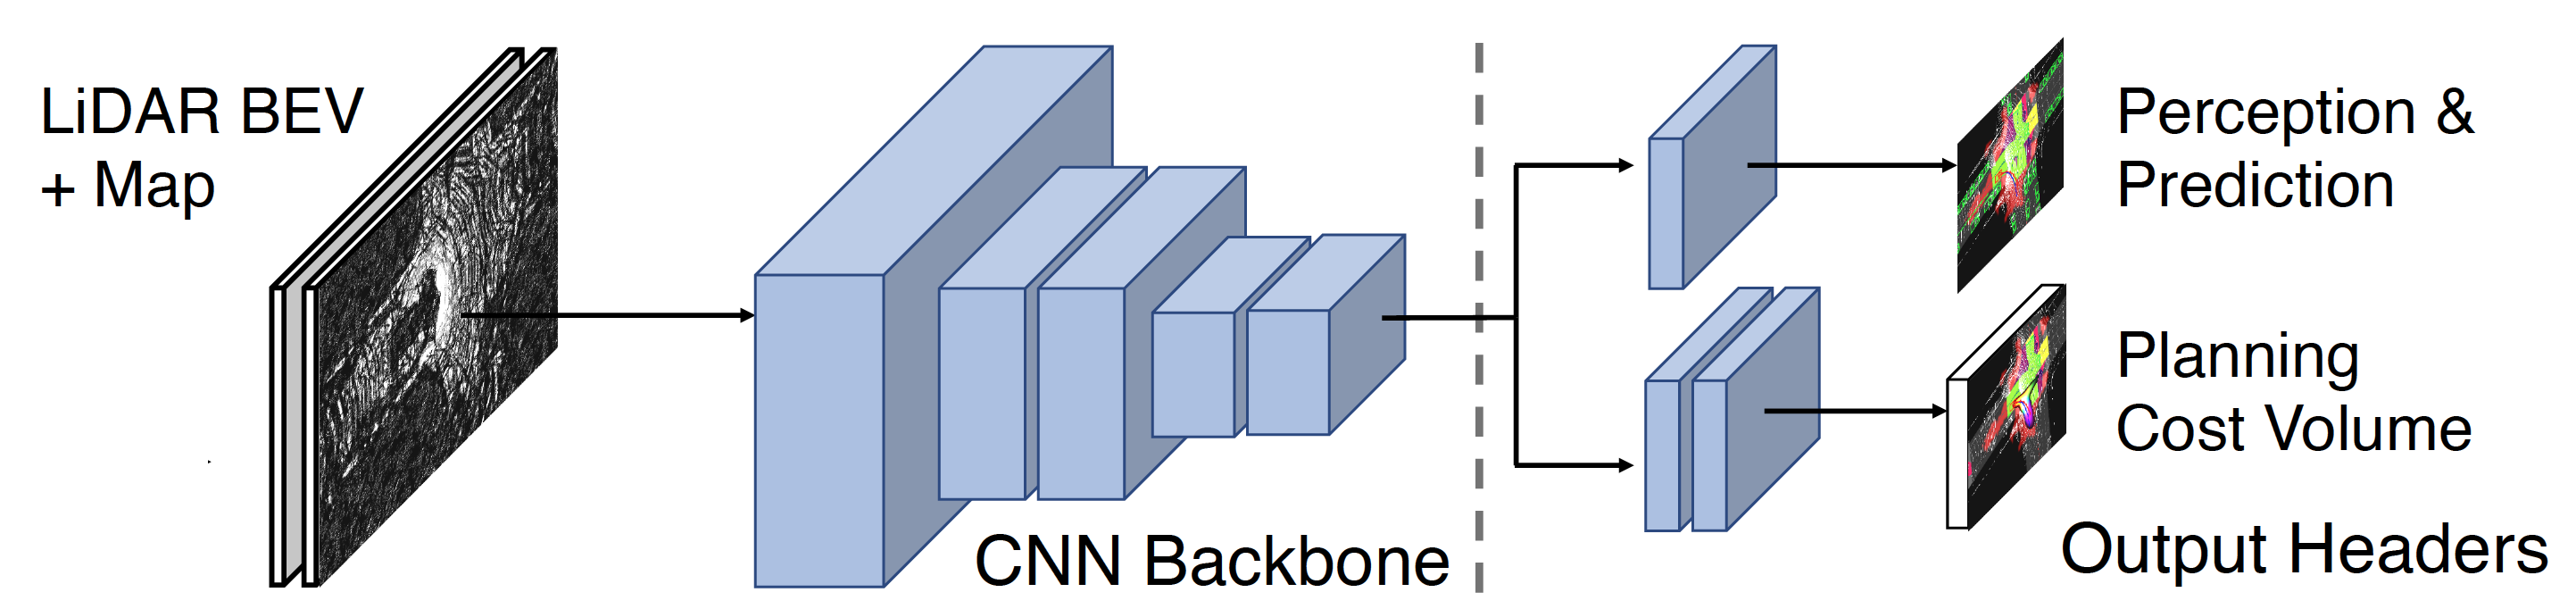
\includegraphics[width=6\textwidth]{figures/nmp2.png}
  \else
  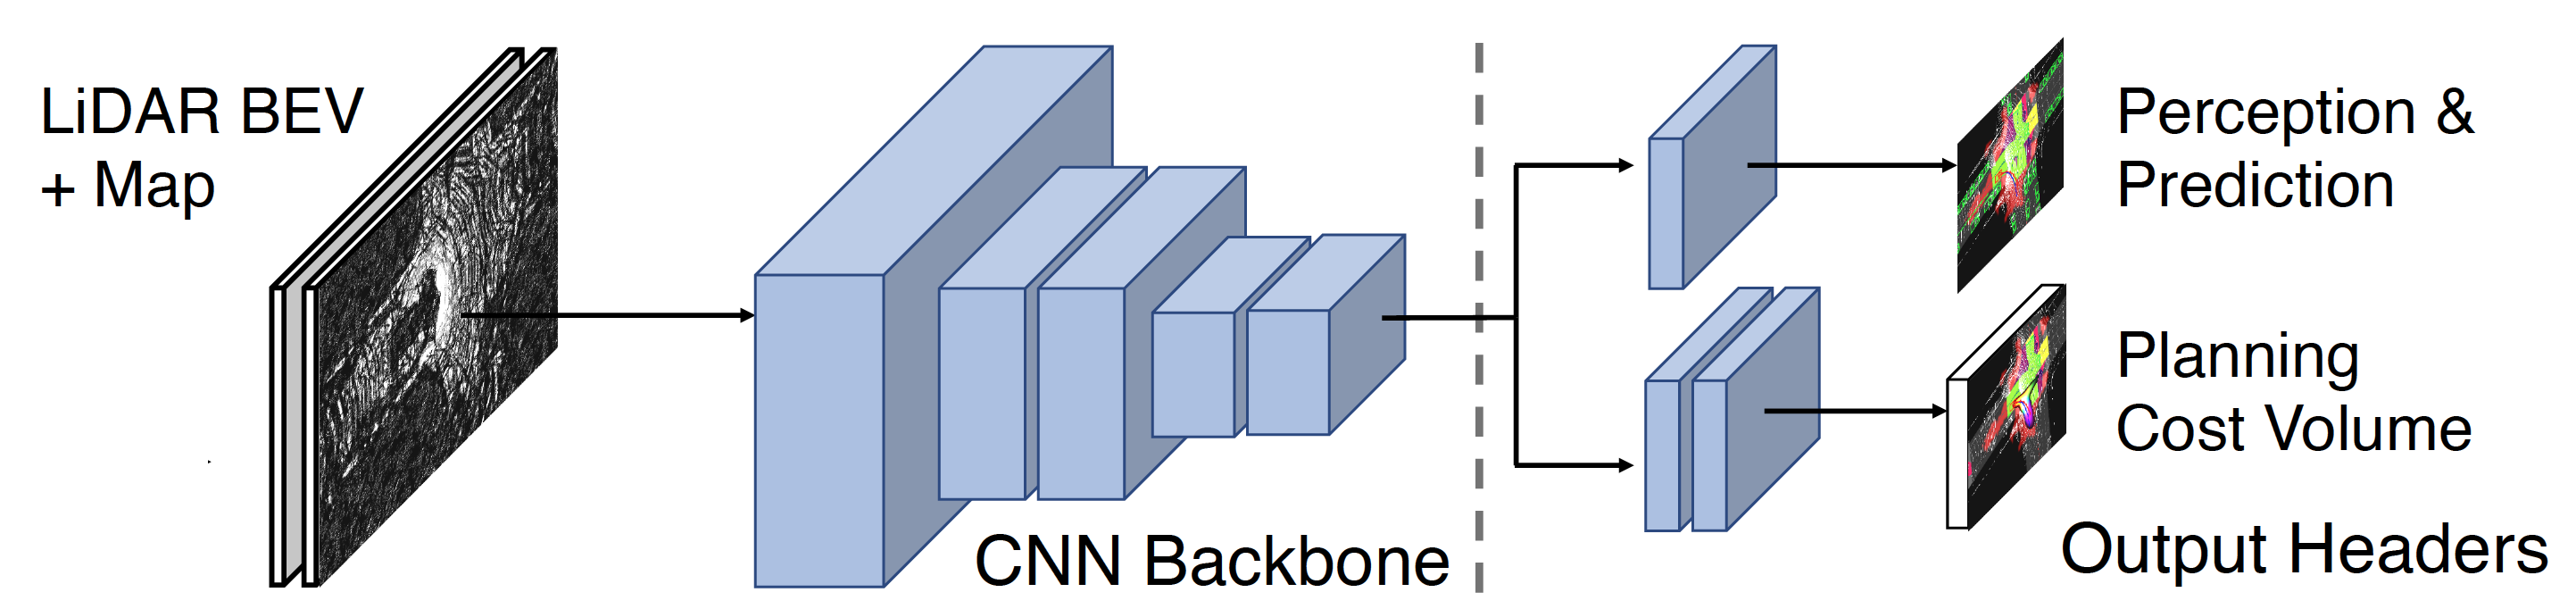
\includegraphics[width=\linewidth,trim={1cm 12.5cm 5cm 0},clip]{figures/nmp2.pdf}
  \fi
  \caption{\small The full neural motion planner (NMP) \cite{nmp} with backbone network and header networks.}
  \label{fig:nmp}
  \vspace{-0.15in}
\end{figure}
\section{Perceive, Attend and Drive}
In this section, we present our framework for using learned, motion-planning aware attention.
We first describe  the end-to-end neural motion planner that serves as the
starting point of our work, and then introduce our proposed attention module and
attention-driven loss function, which enable us to focus the computation in areas that matter for the end task of driving.

\begin{figure}[t]
  \centering
  \iflatexml
  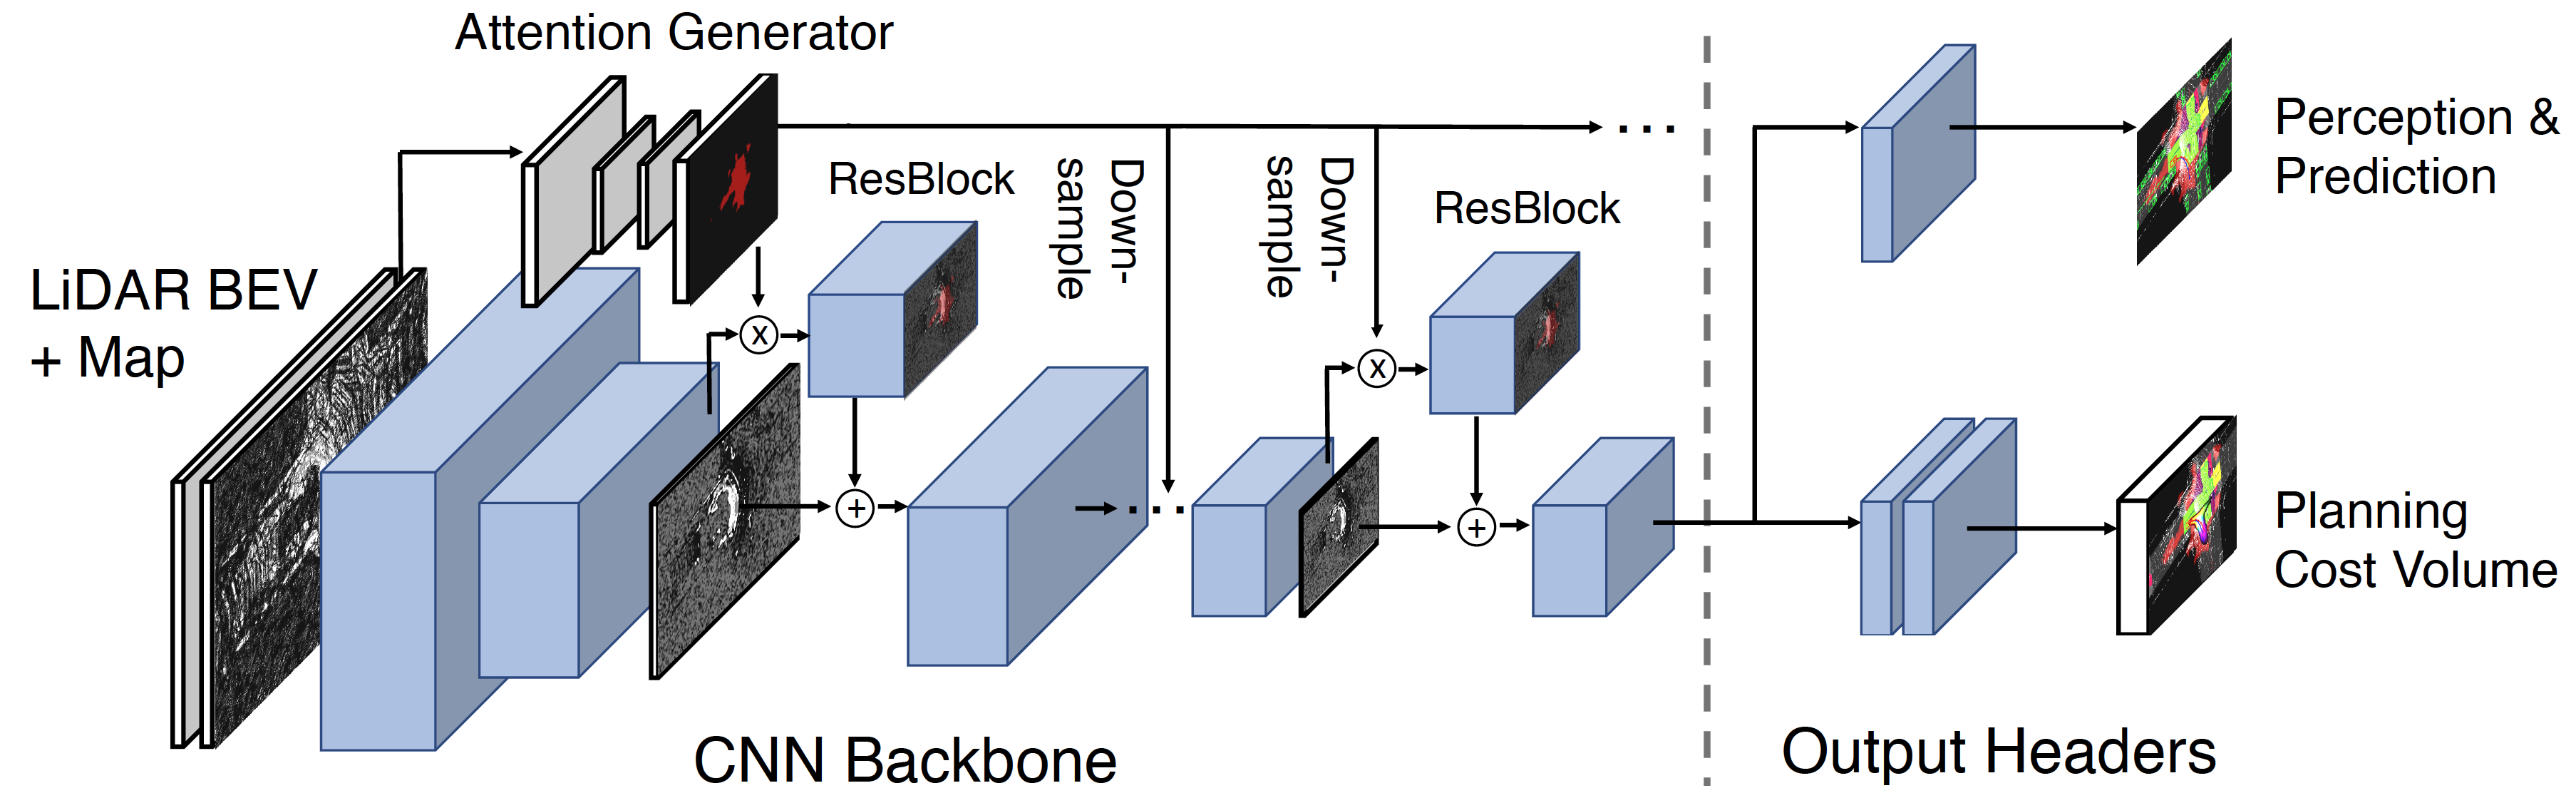
\includegraphics[width=6\textwidth]{figures/sa-nmp2.png}
  \else
  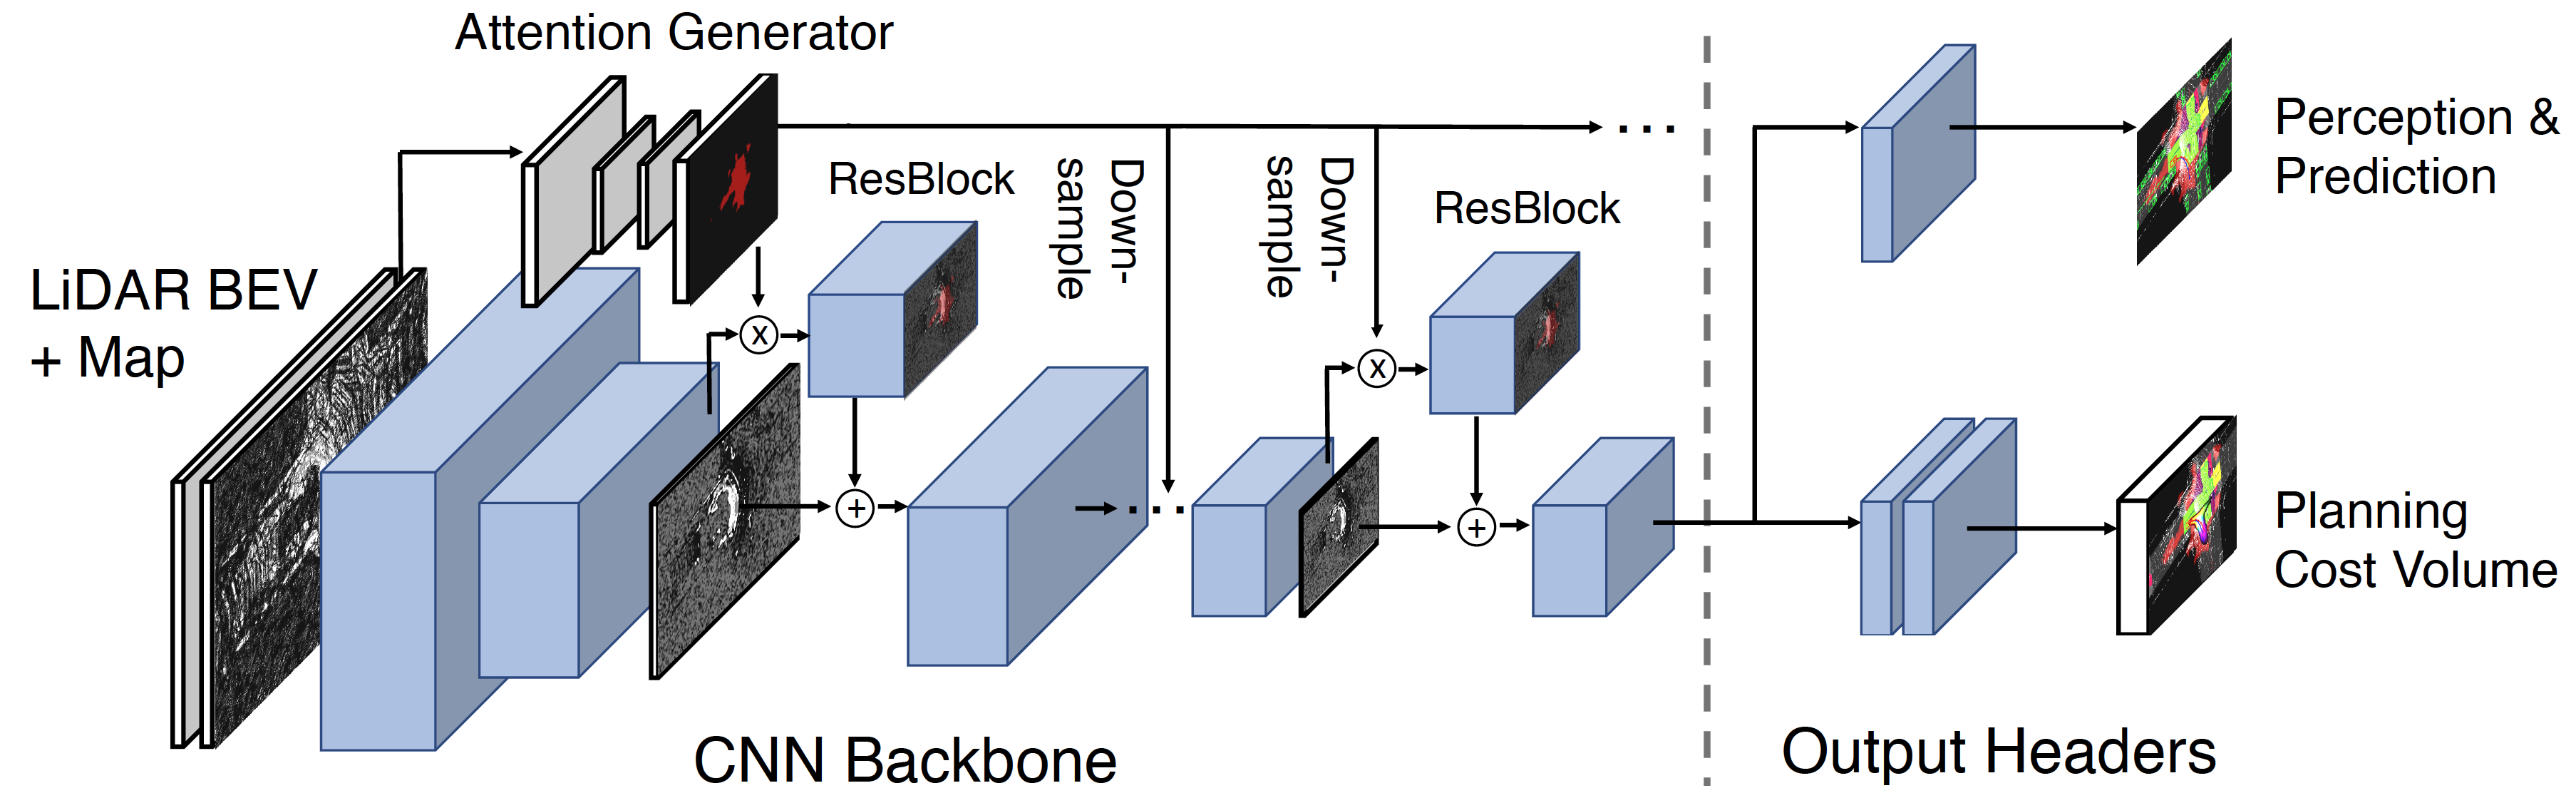
\includegraphics[width=\linewidth,trim={1.2cm 9cm 0 0},clip]{figures/sa-nmp2.pdf}
  \fi
  \caption{\small Our sparse attention neural motion planner (SA-NMP), which takes in LiDAR and HDMaps
  data, and outputs perception, prediction, and planning. Attention is generated from a U-Net and
  applied on the input branches of residual blocks. Our attention is learned towards the planning task, which is a direct model output.}
  \label{fig:mainfig}
  \vspace{-0.15in}
\end{figure}

\subsection{A review on Neural Motion Planner (NMP)}
Our proposed model extends upon the neural motion planner (NMP), which jointly solves the
perception, prediction and planning problems for self-driving. In this section we briefly review NMP depicted in Figure~\ref{fig:nmp}, and refer the reader to ~\cite{nmp} for more details.

\textbf{Input and backbone:} NMP voxelizes LiDAR point clouds to a birds-eye-view (BEV) feature map and fuses them with $M$ channels of rasterized HDMap features to produce an input representation of size $(ZT'+M)\times H\times W$, where $Z,H,W$ are the height and spatial dimensions and $T'=10$ is the number of input LiDAR sweeps. The backbone consists of 5 blocks, with the first 4 producing multi-scale features that are concatenated and fed to the final block. Overall the backbone downsamples the spatial dimension by 4.

\textbf{Multi-task headers:}
Given the features computed by the backbone, $\Inp \in \mathbb{R}^{128\times \frac{H}{4} \times \frac{W}{4}}$, NMP uses two separate headers for perception \& prediction, and motion planning.
 The perception \& prediction header consists of separate branches for classification and regression. The classification branch outputs a score for each anchor box at each spatial location over the feature map $X$, while the regression branch outputs regression targets for each anchor box, including targets for localization offset, size, and heading angle.
The planning header consists of convolution and deconvolution layers to produce a cost volume $ \cC \in \mathbb{R}^{T \times H \times W}$ representing the cost for the self-driving vehicle to be at each location and time, with $T$ the fixed future planning horizon.

\textbf{Planning inference:}
At inference time, NMP samples $N$ trajectories  that are physically realizable, and chooses the lowest cost trajectory for the ego-car:
\vskip -0.15in
\begin{align}
\tau^\star(\Inp) = \argmin_{\tau_{1 \dots N}} \ \ c(\tau_i, \Inp),
\end{align}
% \vskip -0.1in
where the cost of a
trajectory $\tau = (x_t, y_t)_{t=1}^{T}$ is the sum of all waypoints in the cost volume:
\vskip -0.15in
\begin{align}
c(\tau, \Inp) = \sum_{t=1}^T \cC_{t, x_t, y_t}(\Inp).
\end{align}
% \vskip -0.05in
We sample trajectories using a mixture of Clothoid~\cite{clothoid}, circle, and straight curves. We refer the readers to \cite{nmp} for more details on the sampling procedure.

\subsection{Sparse Attention Neural Motion Planner (SA-NMP)}
% \vspace{-0.1in}
In this section, we propose our sparse spatial attention module for self-driving, shown in Fig.~\ref{fig:mainfig}, which learns to save computation while performing well on the end task of driving safely to the goal.

\textbf{Input and backbone:} We exploit the same input representation as NMP and use the same perception, prediction, and planning headers.
The NMP backbone is replaced with the state-of-the-art backbone network of  PnPNet~\cite{pnpnet}, which uses cross-scale blocks throughout to fuse BEV sensory input. Each cross-scale block consists of three parallel branches at different resolutions that downsample the feature map, perform bulk computations, and then upsample back to the backbone resolution, before finally fusing cross-scale features across all branches. There is an additional residual connection across each cross-scale block. The final output feature from the backbone consists of 128 channels at 4$\times$ downsampled resolution, which is forwarded to the planning and detection headers.
In addition to the improved performance, PnPNet can be easily scaled for different computational budgets by varying the depth and width of the cross-scale blocks.

Existing attention-driven approaches~\cite{sbnet} tackle only the perception task and use either a road mask obtained from map information or a vehicle mask produced by a different perception module. As a consequence, they waste computation on areas that will not affect the self-driving car. We instead propose a novel approach that is end-to-end trainable and performs computation selectively for planning a safe maneuver.
As shown in Fig.~\ref{fig:mainfig}, the learned attention mask then gates the backbone network, limiting computation to areas where attention is active. By
using binary attention, we can leverage sparse convolution to improve the computational efficiency.

\textbf{Generating binary attention:}
Computational efficiency has been shown to be one of the most prominent advantages of using the
attention mechanism. For soft attention masks the computation is still dense across the entire
activation map, and therefore no computation savings can be achieved.  SBNet~\cite{sbnet} showed that a sparse convolution operator can achieve significant speed-ups with a given
discrete binary attention mask. Here, we would also like to exploit the computational benefit of
sparse convolution by using discrete attention outputs.

We utilize a network to
predict a scalar score for each spatial location, and binarize the score to represent our sparse attention map. For efficiency and simplicity, we use a small U-Net~\cite{unet} with skip
connections and two downsample/upsample stages.
We would like to apply the generated attention back to the BEV features in the
model backbone so as to sparsify the spatial information, allowing computation to be focused on the
important regions only. We choose to do so in a residual manner~\cite{resattn,sbnet} to avoid
deteriorating the features throughout the backbone. Let $x + F(x)$ denote the normal residual block.
Our attention mask is multiplied with the input to the residual block as follows:
\begin{align}
\mathrm{ResAttend}(x) = x + F(x \odot A),
\end{align}
where $\odot$ denotes elementwise multiplication. See Fig. \ref{fig:mainfig} for an illustration of our architecture.

\textbf{Learning binary attention with Gumbel softmax:}
In order to learn the attention generator and backpropagate through the binary attention map, we make use of the Gumbel
softmax technique \cite{gumbel,concrete} since the step function is not differentiable, and using
the standard sigmoid function suffers from a more severe bias-variance trade-off~\cite{gumbel}. Let
$i,j$ denote spatial coordinates, and $z_{i,j}$ the scalar output from the attention U-Net. We first
add the Gumbel noise on the logits as follows:
\vskip -0.15in
\begin{align}
  \pi_{i,j} &= \sigmoid(z_{i,j}) \\
  \alpha_{i,j}^{(0)} &= \log \pi_{i,j} + g_{i,j}^{(0)}\\
  \alpha_{i,j}^{(1)} &= \log (1 - \pi_{i,j}) + g_{i,j}^{(1)},
\end{align}
where $g_{i,j} = -\log(-\log u)$, and $u$ is sampled from $\textrm{Uniform}[0,1]$. At inference time,
hard attention $A_{i,j}$ can be obtained by comparing the logits,
\begin{align}
\attn_{i,j} &= \begin{cases}
1 & \text{if} \ \ \ \alpha_{i,j}^{(0)} \ge \alpha_{i,j}^{(1)} \\
0 & \text{otherwise}.
\end{cases}
\end{align}
During training, however, we would like to approximate the gradient by using the straight-through
estimator~\cite{gumbel,ste}. Hence, in the backward pass, the step function is replaced with a
softmax function with a temperature constant $\temp$ (where $\sattn$ is the underlying soft attention):
\begin{align}
\sattn_{i,j} &= \frac{\exp \left( \alpha_{i,j}^{(0)}/\temp \right)}
  {\exp\left(\alpha_{i,j}^{(0)} / \temp \right)
   + \exp\left(\alpha_{i,j}^{(1)} / \temp \right)}.
\end{align}

\subsection{Multi-Task Learning}
\label{sec:loss}
We train our sparse  neural motion planner (including the attention) end-to-end with a multi-task learning
objective that combines planning ($\cL_{\text{plan}}$) with perception \& motion forecasting ($\cLcla$, $\cLreg$):
\begin{align}
\cL = \lpln \cLpln + \lcla \cLcla + \lreg \cLreg + \lalp \cLatn + \lambda \lVert w \rVert^2_2,
\label{eq:joint}
\end{align}
where $\cLatn$ is an $\ell_1$ loss, defined in Equation~\ref{eq:regularize}, that controls the sparsity of the attention mask, and $\lVert w
\rVert^2_2$ is the standard weight decay term. Following \cite{nmp, pnpnet}, we fix $\lpln=0.001, \lcla=1.0,
\lreg=0.5$.

\textbf{Motion planning loss:} The motion planning loss utilitizes the max-margin objective, where
the ground-truth driving trajectory (performed by a human) should be of lower cost than other
trajectories sampled by the model. Let $(x_t, y_t)$ be the groundtruth trajectory and let $c_t$ be
the cost volume output by the model for timestamp $t$. We randomly sample $N$ trajectories serving as negative samples: $\{x_t^{(i)}, y_t^{(i)}\}_{i=1}^N$, and  penalize the maximum margin violation between groundtruth and negative samples:
\begin{align}
\cLpln &= \max_{i=1 \dots N} \sum_{t=1}^{T} \max\{ 0, c_t - c^{(i)}_t + \Delta_t^{(i)} \},
\end{align}
where $\Delta^{(i)}_t$ is the task loss capturing spatial differences, and traffic violations denoted by $v$. $v^{(i)}_t$ is non-zero when negative trajectory $i$ violates a traffic rule at time $t$:
\begin{align}
\Delta^{(i)}_t &= \left \lVert (x_t, y_t) - (x^{(i)}_t, y^{(i)}_t) \right \rVert_2 + v^{(i)}_t.
\end{align}

\textbf{Perception \& prediction (PnP) loss:} This loss follows the
standard classification and regression objectives for object detection. The classification part uses binary cross-entropy:
\begin{align}
\hspace{-0.07in}
\cLclaij = \sum_k -\hat{y}_{i,j,k} \log(y_{i,j,k}) - (1- \hat{y}_{i,j,k}) \log (1 - y_{i,j,k}),
\end{align}
where $y$ is the predicted classification score between 0 and 1, and $\hat{y}$ is the binary
ground truth. For each detected instance, the model outputs a bounding box, and a pair of coordinates
and angles for each future step. We reparameterize the shift of a bounding box $(x, y, w, h, \theta)$ from
an anchor bounding box $(x_a, y_a, w_a, h_a, \theta_a)$ in a 6-dimensional vector $\delta$:
\begin{align}
\delta_t = 
[
\frac{x_a - x}{w_a},
\frac{y_a - y}{h_a},
\log \frac{w}{w_a},
\log \frac{h}{h_a},
\sin (\theta_a - \theta),
\cos (\theta_a - \theta)
].
\end{align}
A regression loss is then applied for the trajectory of the instance up to time $T$. For each
spatial coordinate $(i,j)$, we sum up the losses of all bounding boxes $b$ where the ground truth belongs to this location:
\begin{align}
\cLregij = \sum_{b \in (i, j)} \sum_{t=0}^{T} \mathrm{SmoothL1}(\hat{\delta}_{b,t}, \delta_{b,t}),
\end{align}
with $\hat{\delta}$  the predicted shifts and $\delta$  the ground truth shifts.

\textbf{Auxiliary loss masking:} Our overall objective is to achieve good performance
in motion planning, so PnP is an auxiliary task. Since the majority of our
computation happens within the attended area, intuitively the model should not be penalized as
severely for mis-detecting objects not in the attended area. We, therefore, propose to use
our spatial attention mask $A$ to re-weight the PnP losses as follows:
\begin{align}
\cLcla &= \gamma_1 \sum_{i,j} \attn_{i,j} \cLclaij + \gamma_0 \sum_{i,j} \cLclaij,\\
\cLreg &= \gamma_1 \sum_{i,j} \attn_{i,j} \cLregij + \gamma_0 \sum_{i,j} \cLregij,
\label{eq:reweight}
\end{align}
where $\gamma_1$ weights attended instances, and $\gamma_0$ weights all instances. We fix $\gamma_0 = 0.1$ and $\gamma_1 = 0.9$.

\textbf{Attention sparsity loss:}
To encourage focused attention and high sparsity, we use an $\ell_1$ regularizer on the attention mask as follows. We control sparsity with $\lambda_A$ in Equation~\ref{eq:joint}.
\vskip -0.05in
\begin{align}
\cLatn = \sum_{i,j} \attn_{i,j}.
\label{eq:regularize}
\end{align}
\vskip -0.05in